% -*- mode: latex-mode; TeX-engine: xetex; LaTeX-command-style: (("" "SOURCE_DATE_EPOCH=0 %(PDF)%(latex) --shell-escape %S%(PDFout)")); TeX-master: "../dissertation.tex"; -*-

\chapter{Raman Sideband Cooling}
\label{ch:rsc}

\section{Introduction}

\section{Theory}

\ref{fig:na-rsc-schematics}

\begin{figure}
  \centering
  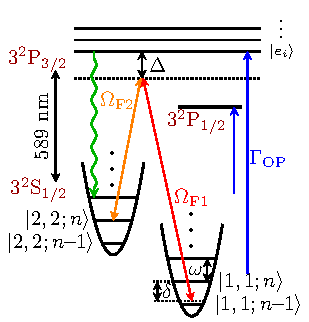
\includegraphics[width=8cm]{figures/na_rsc_schematics.pdf}
  \caption[Schematics of Raman sideband cooling for Sodium.]{
    Single Na atom Raman sideband cooling scheme.
    The Raman transitions between $|2,2;n\rangle$ and $|1,1;n+\Delta n\rangle$
    have a one-photon detuning $\Delta=75$ GHz below the $3^2S_{1/2}$ to $3^2P_{3/2}$ transition.
    Two-photon detuning, $\delta$, is defined relative to the $\Delta n=0$ carrier transition.
    For optical pumping, we use two $\sigma^+$ polarized transitions,
    one to pump the atom state out of $|1,1\rangle$ via $3^2P_{3/2}$
    and one to pump atoms out of $|2,1\rangle$ via $3^2P_{1/2}$
    to minimize heating of the $|2,2\rangle$ state.
    \label{fig:na-rsc-schematics}}
\end{figure}

\section{Setup}

\ref{fig:na-rsc-geometry}

\begin{figure}
  \centering
  \includegraphics[width=8cm]{figures/na_rsc_geometry.pdf}
  \caption[Beams and field geometry for Sodium Raman sideband cooling]{
    Geometry and polarizations of the Raman and optical pumping beams relative to the
    optical tweezer and bias magnetic field.
    Raman beams R1 and R4 address the radial $x$-mode.
    R1 and R2 address the radial $y$-mode.
    R3 and R4 address the axial $z$-mode, where the beams also couple to radial motion,
    but this coupling can be neglected when the atoms is cooled to the ground state of motion.
    \label{fig:na-rsc-geometry}}
\end{figure}

\section{Challenge with Large Lamb-Dicke Parameter}

\ref{fig:na-rsc-challenges}

\begin{figure}
  \centering
  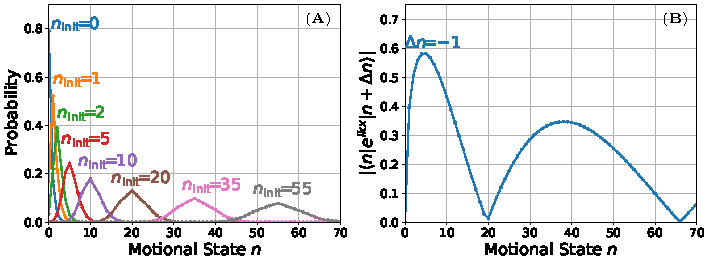
\includegraphics[width=\textwidth]{figures/na_rsc_challenges.pdf}
  \caption[Optical pumping motional-state redistribution and Raman coupling]{
    Optical pumping motional-state redistribution and Raman coupling for large LD parameters
    for the axial direction ($z$).
    The range plotted covers $95$\% of the initial thermal distribution.
    (A) Motional state distribution after one OP cycle for different initial states motion,
    $n_{\textrm{init}}$.
    Due to photon-recoil and the large LD parameter, $\eta^{\textrm{OP}}_z=0.55$,
    there is a high probability of $n$ changing.
    (B) Matrix elements for Raman transition on the first order cooling sideband
    deviate from $\sqrt{n}$ scaling with multiple minima.
    \label{fig:na-rsc-challenges}}
\end{figure}

\section{Solution: High Order Sidebands}

\ref{fig:na-rsc-mele-raman}

\begin{figure}
  \centering
  \includegraphics[width=8cm]{figures/na_rsc_mele_raman.pdf}
  \caption[Raman coupling including high order sidebands]{
    Matrix elements for Raman transition including high order sidebands.
    During cooling, we utilize the fact that high motional states couple most effectively
    to sidebands with large $|\Delta n|$ in order to overcome the issue with
    variation and dead zone in the coupling strengths.
    \label{fig:na-rsc-mele-raman}}
\end{figure}

\section{Solution: Simulation Based Optimization}

\ref{fig:na-rsc-sequence}

\begin{figure}
  \centering
  \includegraphics[width=\textwidth]{figures/na_rsc_sequence.pdf}
  \caption[Simulation optimized Raman sideband cooling sequence for Sodium]{
    Schematic of the cooling pulse sequence. The tweezer is strobed at 3 MHz to
    reduce light shifts during optical pumping\todo{~\cite{Hutzler2017-LightShifts}}.
    Each cooling cycle consists of $8$ sideband pulses.
    The four axial pulses address two sideband orders.
    The two pulses in each radial direction either address $\Delta n=-2$ and $\Delta n=-1$
    or have different durations to drive $\Delta n=-1$,
    at the end of the cooling sequence when most of the population is below $n=3$.
    The Raman cooling and spectroscopy pulses have Blackman envelopes\todo{~\cite{Kasevich1992}}
    to reduce off-resonant coupling,
    while the measurement Rabi pulses in Fig.~\ref{fig:na-rsc-rabi-flop}
    have square envelopes to simplify analysis.
    \label{fig:na-rsc-sequence}}
\end{figure}

\section{Cooling Performance}

\ref{fig:na-rsc-spectrum}
\ref{fig:na-rsc-rabi-flop}

\begin{figure}
  \centering
  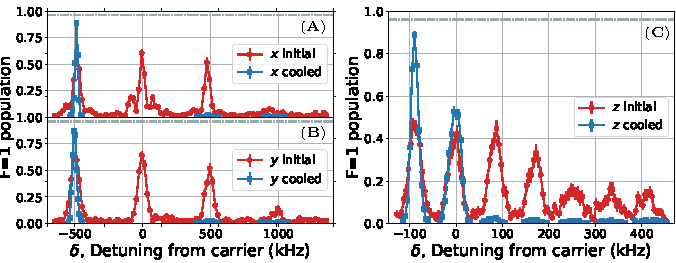
\includegraphics[width=\textwidth]{figures/na_rsc_spectrum.pdf}
  \caption[Raman sideband spectra before and after cooling]{
    Raman sideband spectra for (A) $x$, (B) $y$, (C) $z$ axis before (red circle)
    and after (blue square) applying Raman sideband cooling sequence.
    The height of the cooling sidebands (positive detuning)
    are strongly suppressed after cooling which suggests most of the atoms are cooled
    to the motional ground state in the trap.
    \label{fig:na-rsc-spectrum}}
\end{figure}

\begin{FPfigure}
  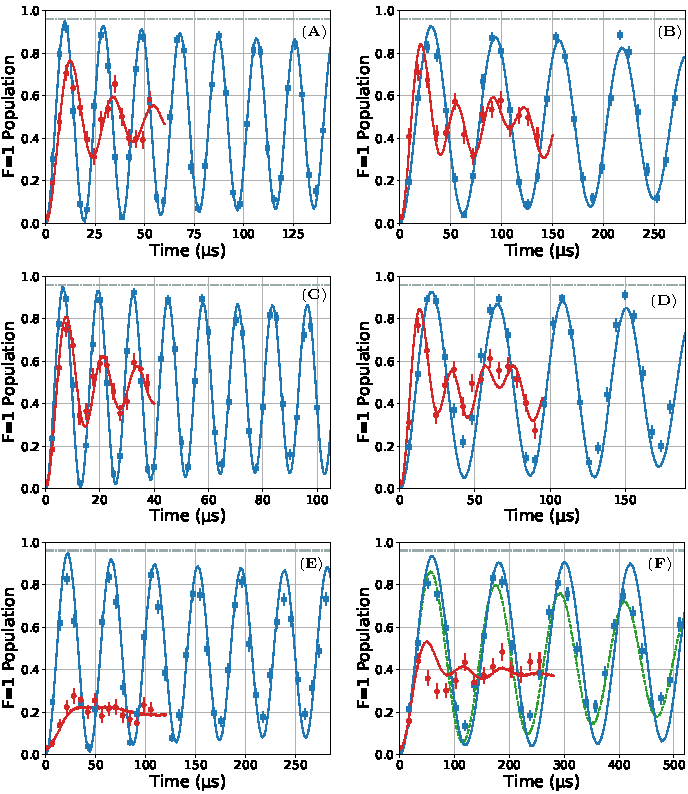
\includegraphics[width=\textwidth]{figures/na_rsc_rabi_flop.pdf}
  \caption[Rabi flopping on carriers and sidebands]{
    Rabi flopping on radial axis $x$ (A) carrier and (B) $\Delta n_x=1$ sideband,
    radial axis $y$ (C) carrier and (D) $\Delta n_x=1$ sideband,
    axial axis $z$ (E) carrier and (F) $\Delta n_x=1$ sideband,
    before (red circle) and after (blue square) Raman sideband cooling.

    Solid lines (both red and blue) in all plots are fits to a Rabi-flopping
    that includes a thermal distribution of motional states\todo{~\cite{Meekhof1996}}
    as well as off-resonant scattering from the Raman beams.

    The blue lines correspond to a ground state probability of (A-D) $98.1$\% along radial axis
    and (E-F) $95$\% along the axial axis after cooling.
    The red lines correspond to a thermal distribution of $80$ $\mu$K before RSC.
    The horizontal dashed lines in all the plots correspond to the $4\,\%$ probability
    of imaging loss.

    The green dashed line in (F) includes the additional decoherence due to
    a fluctuation of the hyperfine splitting of magnitude $3$ kHz.
    We see that the decoherence effect is strongest for the post-cooling data on
    the axial $\Delta n_z=1$ sideband where the Rabi frequency is the lowest.
    \label{fig:na-rsc-rabi-flop}}
\end{FPfigure}
\afterpage{\clearpage}
